\documentclass{article}
\usepackage[normalem]{ulem}
\usepackage[14pt]{extsizes}
\usepackage[utf8]{inputenc}
\usepackage[T2A]{fontenc}
\usepackage{amsmath}
\usepackage{amssymb}
\usepackage{mathtools}
\usepackage{hyperref}
\usepackage{amsfonts}
\usepackage{cmap}
\usepackage{multicol}
\usepackage{comment}
\usepackage[parfill]{parskip}

\usepackage{listings}
\usepackage{color}
\usepackage{colortbl}
\usepackage{xcolor}
\usepackage[left=1.5cm,right=2cm,top=2cm,bottom=2cm,bindingoffset=0.1cm]{geometry}
\usepackage[russian]{babel}
\usepackage[pdf]{graphviz}
\usepackage{tikz}
\usepackage{pgfplots}
\usepgfplotslibrary{polar}
\usepackage{etoolbox} % <--- added
\AtBeginEnvironment{enumerate}{\linespread{.84}\selectfont}
\newcommand{\ctd}{\begin{flushright} $\square$ \end{flushright}}
%%% Работа с картинками
\usepackage{graphicx}  % Для вставки рисунков
  % папки с картинками
\setlength\fboxsep{3pt} % Отступ рамки \fbox{} от рисунка
\setlength\fboxrule{1pt} % Толщина линий рамки \fbox{}
\pagenumbering{gobble}

\hypersetup{
    colorlinks=true,
    linkcolor=blue,
    filecolor=magenta,      
    urlcolor=blue,
    pdftitle={Alfo},
    pdfpagemode=FullScreen,
    }
\lstset{ %
  language=C++, % the language of the code
  basicstyle=\footnotesize\ttfamily, % the size of the fonts that are used for the code
  numbers=left, % where to put the line-numbers
  numberstyle=\footnotesize\color{black},  % the style that is used for the line-numbers
  stepnumber=0, % the step between two line-numbers. If it's 1, each line 
       % will be numbered
  numbersep=0.7em,       % how far the line-numbers are from the code
  backgroundcolor=\color{white!95!gray}, % choose the background color. You must add \usepackage{color}
  showspaces=false,      % show spaces adding particular underscores
  showstringspaces=false,% underline spaces within strings
  showtabs=false,        % show tabs within strings adding particular underscores
  frame=single, % adds a frame around the code
  rulecolor=\color{black},        % if not set, the frame-color may be changed on line-breaks within not-black text (e.g. commens (green here))
  tabsize=2,    % sets default tabsize to 2 spaces
  %captionpos=b,% sets the caption-position to bottom
  breaklines=true,       % sets automatic line breaking
  breakatwhitespace=false,        % sets if automatic breaks should only happen at whitespace
  %title=\lstname,       % show the filename of files included with \lstinputlisting;
       % also try caption instead of title
  identifierstyle=\color{black!50!green},  
  keywordstyle=\color{blue},      % keyword style
  commentstyle=\color{gray},      % comment style
  stringstyle=\color{purple},      % string literal style
  escapeinside={\%*}{*)},% if you want to add a comment within your code
  morekeywords={n,k},    % if you want to add more keywords to the set
  morecomment=[l][\color{black!50!green}]{\#}, % to color #include<cstdio> 
  morecomment=[s][\color{gray!50!black}]{/**}{*/}
}

\usepackage{amsmath,amssymb}
\usepackage{ stmaryrd }
\usepackage{ dsfont }
\usepackage{ tipa }
\usepackage{tocloft}

\newcommand{\updownarrows}{\mathbin\uparrow\hspace{-.5em}\downarrow}
\newcommand{\downuparrows}{\mathbin\downarrow\hspace{-.5em}\uparrow}
\newcommand{\defeq}{\stackrel{\mathclap{\normalfont\mbox{def}}}{=}}
\newcommand{\defLeftrightarrow}{\xLeftrightarrow{def}}

\usepackage{pgfplots}
\pgfplotsset{compat=1.9}

\makeatletter
\renewcommand*\env@matrix[1][*\c@MaxMatrixCols c]{%
  \hskip -\arraycolsep
  \let\@ifnextchar\new@ifnextchar
  \array{#1}}
\makeatother


\title{Линейные пространства и все об этом. Линейная Алгебра}
\author{Чепелин В.А.}
\date{}

\begin{document}
\maketitle
\tableofcontents
\pagebreak
\section{Введение.}

 Здесь содержатся мое объяснение задач по лин пространствам из  кр по лин. алу. Тут вы сможете понять что как решать. Списывать плохо!!! Всем счастья!
\begin{center}
   
\includegraphics[width=12.65cm, height=18cm]{аниме.jpg}
\end{center}

\section{Матрица перехода и все об этом.}

\subsection{Определение.}

Начнем с определения. \textbf{Что же такое эта ваша матрица перехода?}

Давайте зафиксируем старый базис $E = (e_1,e_2,\ldots e_n)$. Для каждого вектора этого базиса мы знаем его координаты в этом базисе. Например $X= 
\begin{pmatrix}
    x_1\\
    x_2\\
    \vdots\\
    x_n\\
\end{pmatrix}
$

Теперь я хочу ввести новый базис $E' = (e_1',e_2',\ldots,e_n')$.  

И теперь у меня возникает желание переводить огромное количество векторов  из старого базиса в новый.

Давайте разложим каждый вектор нового базиса через старый и пусть $e_1' = T_1, e_2' = T_2, \ldots. e_n = T_n$, где $T_i$ - представление i-ого вектора в этом базисе, тогда:

$T=(T_1, T_2,\ldots, T_n) = T_{e\rightarrow e'}$ - \textbf{матрица перехода} из e в e', причем:

$E \cdot  T_{e\rightarrow e'} = E' $, что можно заметить из соответсвующего произведения столбиков и строчек. Теперь поймем как нам с помощью этой матрицы быстро переводить из одного базиса в другой:

$ T_{e\rightarrow e'} \cdot x' = x$ - матрица перехода умноженная на представление в новом базисе = вектор в старом базисе. 

\subsection{Примерчики.}
Давайте рассмотрим это на очень простеньких примерах.

1) Например мы хотим из канонического базиса в $R^3$ перейти  в базис вот таких векторов:$\begin{pmatrix}
    0\\
    0\\
    1\\
\end{pmatrix}$ $\begin{pmatrix}
    0\\
    1\\
    0\\
\end{pmatrix}$ $\begin{pmatrix}
    1\\
    0\\
    0\\
\end{pmatrix}$
\sout{невероятный базис совсем не похожий на канонический честно}.

Тогда напишем представление этих векторов через канонический. Шок это он и будет, тогда напишем матрицу перехода:

$T_{e \rightarrow e'} = \begin{pmatrix}
    0 & 0 & 1\\
    0 & 1 & 0\\
    1 & 0 & 0\\
\end{pmatrix}$
И теперь давайте представим вектор $ \begin{pmatrix}
    1000 \\
    993 \\
    986 \\
\end{pmatrix}$ в новом базисе.

По определению:

$T_{e \rightarrow e'} x' = \begin{pmatrix}
    1000 \\
    993  \\
    986  \\
\end{pmatrix} $ или  $ \begin{pmatrix}
    0 & 0 & 1\\
    0 & 1 & 0\\
    1 & 0 & 0\\
\end{pmatrix}x' = \begin{pmatrix}
    1000  \\
    993  \\
    986  \\
\end{pmatrix} $

По-хорошему здесь решать систему (об этом позже), но мои супер глаза и так видят ответ: $x' =  \begin{pmatrix}
    986 \\
    993  \\
    1000  \\
\end{pmatrix} $

\sout{Задача на самом деле имеет глубокий подтекст. Канеки Кен теперь не вычитает из 1000 7, а прибавляет, поэтому он здоров, а не психически болен. Лин. ал лечит}

2) Например мы хотим из вот такого базиса: $\begin{pmatrix}
    1\\
    2\\
    3\\
\end{pmatrix}$ $\begin{pmatrix}
    1\\
    1\\
    1\\
\end{pmatrix}$ $\begin{pmatrix}
    0\\
    1\\
    1\\
\end{pmatrix}$ в $R^3$ перейти  в канонический базис. 

Напишем представление каждого канонического базиса через этот. Давайте решать уравнения:


Надо найти:

$T_1,T_2, T_3$ - вектора в старом базисе, соответсвующую новому вектору(хотим новый базис через старый представить)

$T_1 = \begin{pmatrix}
    t_{11} \\ 
    t_{12} \\ 
    t_{13} \\ 
\end{pmatrix}$ $\ldots$ $T_3 = \begin{pmatrix}
    t_{31} \\ 
    t_{32} \\ 
    t_{33} \\ 
\end{pmatrix}$

Получается, что $E\cdot T_1 = e_1$; $E\cdot T_2 = e_2$; $E\cdot T_3 = e_3$, я должен решить 3 уравнения:

$
\begin{pmatrix}[ccc|c]
   1 &1 &0&1   \\
    2 &1 &1&0 \\
    3& 1&1&0
\end{pmatrix}$
$
\begin{pmatrix}[ccc|c]
   1 &1 &0&0   \\
    2 &1 &1&1 \\
    3& 1&1&0
\end{pmatrix}$
$
\begin{pmatrix}[ccc|c]
   1 &1 &0&0   \\
    2 &1 &1&0 \\
    3& 1&1&1
\end{pmatrix}$

Но решать их 3 по очереди кринге, легче вот так:

$
\begin{pmatrix}[ccc|ccc]
   1 &1 &0&1 & 0 & 0  \\
    2 &1 &1&0 & 1 & 0\\
    3& 1&1&0 & 0 & 1
\end{pmatrix}$

Поэтому все что нам надо - привести левую матрицу в единичную и мы получим матрицу перехода из старого в новый(в правой части). Решаем такое уравнение как бы для сразу для трех переменных (надо привести левую часть в вид единичной матрицы)

Получаем вот такую матрицу перехода:

$T_{e \rightarrow e'} = \begin{pmatrix}
    0 & -1 & 1\\
    1 & 1 & -1\\
    -1 & 2 & -1\\
\end{pmatrix}$

А уже с ее помощью можно находить разные вектора.

\pagebreak

\section{Объединение и пересечение}

\subsection{Теория и примерчики}
\textbf{\uline{Объединение}} - $L_1 + L_2$ - буквально все вектора задаваемые суммой этих двух. Пример - 2 прямых на плоскости(проходящих через ноль и не параллельных) зададут любую точку на этой плоскости. Для них $L_1 + L_2$ - вот эта плоскость


\textbf{\uline{Пересечение}} - $L_1 \cap L_2$ - все вектора, которые буквально лежат в пересечении - Пример - пересечение двух плоскостей по прямой. В таком случае прямая будет для них пересечении

Также для самопроверки мы должны знать:

$\dim (L_1 + L_2) = \dim L_1 + \dim L_2 - \dim (L_1 \cap L_2)$ - \textbf{формула Грассмана}

\pagebreak
\section{Прямая сумма и немного о ней.}

\subsection{Прямая сумма.}
Сумма подпространств называется \textbf{прямой суммой}, если они дизъюнктивны. \sout{Какие-то умные слова пошли.} Теперь на языке адекватном:

Вот у вас есть $L_1, L_2$ и если у вас ранг суммы равен сумме рангов $L_1, L_2$. Например:

$L_1 =spam ( \begin{pmatrix}

    1 \\
    0 \\
    0 \\
    0 
\end{pmatrix}  \begin{pmatrix}
    0 \\
    1 \\
    1 \\
    0 
\end{pmatrix} )$;
$L_2 =spam ( \begin{pmatrix}
    0 \\
    0 \\
    1 \\
    0 
\end{pmatrix}  \begin{pmatrix}
    1 \\
    1 \\
    0 \\
    1 
\end{pmatrix} )$

$rg L_1 = 2; rg L_2 = 2; rg L_1 + rg L_2 = 4$, откуда $L_1 + L_2 = L_1 \oplus L_2 $ --- прямая сумма (обозначение)
\subsection{Проекции.}

Посмотрим на базис прямой суммы. Будем дальше рассматривать все на примерчике сверху (см. прошлый пункт).

$L_1 \oplus L_2  = spam (L_1,L_2) = spam (\begin{pmatrix}
    0 \\
    0 \\
    1 \\
    0 
\end{pmatrix}  \begin{pmatrix}
    1 \\
    1 \\
    0 \\
    1 
\end{pmatrix}\begin{pmatrix}
    1 \\
    0 \\
    0 \\
    0 
\end{pmatrix}  \begin{pmatrix}
    0 \\
    1 \\
    1 \\
    0 
\end{pmatrix})$ 

Хотим найти проекцию вектора $x = \begin{pmatrix}
    3 \\
    4 \\
    1 \\
    7 
\end{pmatrix}$

Давайте сначала построим матрицу перехода в новый базис - базис прямой суммы 

$
T_{e \rightarrow e'}=
\begin{pmatrix}
    0 & 1 &1&0\\
    0 &1&0&1\\
    1 &0&0&1\\
    0 &1&0&0
\end{pmatrix}$

Теперь давайте  найдем вектор x', который соответсвует x в новом базисе(базисе прямой суммы).

$x' = \begin{pmatrix}
    4\\
    7\\
    -4\\
    -3\\
\end{pmatrix}$

Теперь проекция на $L_1$ это вектор $x_1'=\begin{pmatrix}
    4\\
    7\\
    0\\
    0
\end{pmatrix}, $ а на $L_2$ это вектор $x_2'=\begin{pmatrix}
    0\\
    0\\
    -4\\
    -3
\end{pmatrix}$.

Теперь представим их в искомом базе $x_1 = \begin{pmatrix}
    7\\
    7\\
    4\\
    7\\
\end{pmatrix}$, $x_2 = \begin{pmatrix}
    -4\\
    -3\\
    -3\\
    0\\
\end{pmatrix}$.

В таком случае $x_1$ - проекция на $L_1$ вектора x, а $x_2$ - проекция на $L_2$ вектора.

\pagebreak
\section{Задачи с контрольной}

\subsection{Задача на сумму и пересечение.}

Тут будет пример решения одной из задач:

Найти пересечение и сумму:

$L_1 = spam (\begin{pmatrix}
    2 \\
    -2 \\
    0 \\
    -1 \\
\end{pmatrix}, \begin{pmatrix}
    1 \\
    -1 \\
    -1\\
    -1 \\
\end{pmatrix}, \begin{pmatrix}
    3 \\
    -2 \\
    1\\
    1 \\
\end{pmatrix})$

$L_2 = spam (\begin{pmatrix}
    3 \\
    1 \\
    1 \\
    4 \\
\end{pmatrix}, \begin{pmatrix}
    2 \\
    0 \\
    1\\
    5 \\
\end{pmatrix}, \begin{pmatrix}
    1 \\
    -1 \\
    0\\
    1 \\
\end{pmatrix})$

Найдем базис $L_1$:

$rg \begin{pmatrix}
    2 &1 &3 \\
    -2 & -1 & -2 \\
    0 & -1 & 1 \\
    -1 & -1 & 1
\end{pmatrix} = rg \begin{pmatrix}
    0 &0 &1 \\
    -2 & -1 & -2 \\
    0 & -1 & 1 \\
    -1 & -1 & 1
\end{pmatrix} = rg \begin{pmatrix}
    -2 & -1  \\
    0 & -1  \\
    -1 & -1 
\end{pmatrix} + 1 = 3$

Откуда базис $L_1$ это $A_1, A_2, A_3$. 

Найдем базис $L_2$:

$rg \begin{pmatrix}
    3 &2 &1 \\
    1 & 0 & -1 \\
    1 & 1 & 0 \\
    4 & 5 & 1
\end{pmatrix} =rg \begin{pmatrix}
    3 &2 &1 \\
    1 & 0 & -1 \\
    1 & 1 & 0 \\
    1 & 3 & 0
\end{pmatrix} =rg \begin{pmatrix}
    3 &2 &1 \\
    1 & 0 & -1 \\
    1 & 1 & 0 \\
    0 & 2 & 0
\end{pmatrix} = rg \begin{pmatrix}
    3  &1 \\
    1  & -1 \\
    1 & 0 \\
\end{pmatrix} +1 = 3 $

Откуда базис $L_2$ это $B_1, B_2, B_3$. (обозвал ашками и бешками искомые вектора, если кто не понял).

1) {Найдем $L_1+L_2$ и его базис:}

$rg \begin{pmatrix}
    2 &1 &3 & 3 & 2 &1\\
    -2 & -1 & -2 & 1 & 0 &-1\\
    0 & -1 & 1 & 1 & 1 & 0\\
    -1 & -1 & 1 & 4 & 5 & 1
\end{pmatrix} = rg \begin{pmatrix}
    2 &4 &3 & 3 & 2 &1\\
    -2 & -3 & -2 & 1 & 0 &-1\\
    0 & 0 & 1 & 1 & 1 & 0\\
    -1 & 0 & 1 & 4 & 5 & 1
\end{pmatrix} = rg \begin{pmatrix}
    2 &4 &3 & 3 & 2 &1\\
    0 & 1 & 1 & 4 & 2 &0\\
    0 & 0 & 1 & 1 & 1 & 0\\
    -1 & 0 & 1 & 4 & 5 & 1
\end{pmatrix}= rg \begin{pmatrix}
    3 &4 &3 & 3 & 2 &1\\
    0 & 1 & 1 & 4 & 2 &0\\
    0 & 0 & 1 & 1 & 1 & 0\\
    0 & 0 & 1 & 4 & 5 & 1
\end{pmatrix} = 1 +rg \begin{pmatrix}
 1 & 1 & 4 & 2 &0\\
 0 & 1 & 1 & 1 & 0\\
 0 & 1 & 4 & 5 & 1
\end{pmatrix} = 2 +  rg \begin{pmatrix}
1 & 1 & 1 & 0\\
1 & 4 & 5 & 1
\end{pmatrix} = 4 $

Ну и не трудно заметить, что $A_1,A_2,A_3,B_1$ - базис $L_1+L_2$.

2) {Найдем $L_1\cap L_2$ и его базис:}

Посмотрим на какой-то вектор пересечения: 

$x = \alpha_1 A_1 + \alpha_2 A_2 + \alpha_3 A_3 = \beta_1 B_1 + \beta_2 B_2 + \beta_3 B_3$.

Откуда любой вектор пересечения задается

$\alpha_1 A_1 + \alpha_2 A_2 + \alpha_3 A_3 - \beta_1 B_1 - \beta_2 B_2 - \beta_3 B_3 = 0$

Решим систему:

$\begin{pmatrix}[cccccc|c]
    2 &1 &3 & -3 & -2 &-1 &0\\
    -2 & -1 & -2 & -1 & 0 &1 &0\\
    0 & -1 & 1 & -1 & -1 & 0&0\\
    -1 & -1 & 1 & -4 & -5 & -1&0
\end{pmatrix}$

Ее общее решение: $\begin{pmatrix}
    \alpha_1 \\
    \alpha_2 \\
    \alpha_3 \\
    \beta_1 \\
    \beta_2 \\
    \beta_3
\end{pmatrix} = t_2 \begin{pmatrix}
   -\cfrac{11}{2} \\
    \cfrac{5}{2} \\
    4 \\
    \cfrac{1}{2} \\
    1 \\
    0
\end{pmatrix} +  t_3 \begin{pmatrix}
   -\cfrac{5}{2} \\
    \cfrac{3}{2} \\
    2 \\
    \cfrac{1}{2} \\
    0 \\
    1
\end{pmatrix}$

Тогда $\beta_1 = \cfrac{1}{2}t_2 + \cfrac{1}{2}t_3$, $\beta_2 = t_2$,$\beta_3 = t_3$.  Тогда любой x в пересечении задается:

$x = \cfrac{1}{2}t_2 B_1 + \cfrac{1}{2}t_3 B_1 + t_2 B_2 + t_3 B_3 = t_2(\cfrac{1}{2} B_1 + B_2) + t_3 (\cfrac{1}{2} B_1 + B_3)$.

Откуда получаю базис пересечения:

$P_1 = \cfrac{1}{2} B_1 + B_2$, $P_2 = (\cfrac{1}{2} B_1 + B_3)$

\pagebreak

\pagebreak

\subsection{Задача на прямую сумму.}

Условие: 

$L_1$ задано системой 
$
\begin{cases}
    x_1-x_2-x_3+x_4=0\\
    x_1 + 7x_2 + x_3 - 6 x_4 = 0
\end{cases}
$

$L_2$ задано системой 
$
\begin{cases}
   -2x_1=x_2 +x_3\\
   -2x_1 = x_4 \\
\end{cases}
$

Доказать, что $\mathbb{R}^4  = L_1 \oplus L_2$, а также найти проекцию $x = \begin{pmatrix}
    1\\
    10\\
    1\\
    8
\end{pmatrix}$.

1) Найдем базис и ранг $L_1$:

Для этого нам надо решить систему:  
$\begin{pmatrix}[cccc|c]
    1 & -1 & -1 & 1 & 0\\
    1 & 7 & 1 & -6 & 0 \\
\end{pmatrix}$

$X = t_3\begin{pmatrix}
    3\\
    -1\\
    4 \\
    0
\end{pmatrix} + t_4\begin{pmatrix}
    -1\\
    7\\
    0 \\
    8
\end{pmatrix}$

Откуда $L_1 = spam (\begin{pmatrix}
    -1\\
    7\\
    0 \\
    8
\end{pmatrix}, \begin{pmatrix}
    3\\
    -1\\
    4 \\
    0
\end{pmatrix} )$.

2) Найдем базис и ранг $L_2$:   

Решим соответсвующую систему:

$
\begin{cases}
   -2x_1=x_2 +x_3\\
   -2x_1 = x_4 \\
\end{cases}
$

$
\begin{pmatrix}[cccc|c]
    -2 & -1 & -1 & 0 & 0 \\
    -2 & 0 & 0 & -1 & 0 \\
\end{pmatrix} 
$

$X = t_3\begin{pmatrix}
    0\\
    -1\\
    1\\
    0
\end{pmatrix}  + t_4 \begin{pmatrix}
    -1\\
    2\\
    0\\
    2
\end{pmatrix}$

Откуда $L_2  = spam(\begin{pmatrix}
    0\\
    -1\\
    1\\
    0
\end{pmatrix}, \begin{pmatrix}
    -1\\
    2\\
    0\\
    2
\end{pmatrix})$

3) Посмотрим на сумму:

Найдем ранг: $rg \begin{pmatrix}
    -1 & 3 & 0 & -1 \\
    7 & -1 & -1 & 2 \\
    0 & 4 & 1 & 0 \\
    8 & 0 & 0 & 2
\end{pmatrix} = rg \begin{pmatrix}
    -1 & 3 & 0 & -1 \\
    7 & -1 & -1 & 2 \\
    0 & 4 & 1 & 0 \\
    1 & 1 & 1 & 0
\end{pmatrix}  =rg \begin{pmatrix}
    -1 & 3 & 0 & -1 \\
    8 & 0 & 0 & 2 \\
    0 & 4 & 1 & 0 \\
    1 & 1 & 1 & 0
\end{pmatrix}=rg \begin{pmatrix}
    -1 & 3 & 0 & -1 \\
    4 & 0 & 0 & 1 \\
    0 & 4 & 1 & 0 \\
    1 & 1 & 1 & 0
\end{pmatrix}=rg \begin{pmatrix}
    3 & 3 & 0 & 0 \\
    4 & 0 & 0 & 1 \\
    0 & 4 & 1 & 0 \\
    1 & 1 & 1 & 0
\end{pmatrix}=rg \begin{pmatrix}
    1 & 1 & 0 & 0 \\
    4 & 0 & 0 & 1 \\
    0 & 4 & 1 & 0 \\
    0 & 0 & 1 & 0
\end{pmatrix} = 4 $

О как же так?!?!?! $L_1$ и $L_2$ ДИЗЪЮНКТИВНЫ, поэтому $L_1 + L_2 = L_1 \oplus L_2$ 

4) Найдем проекции:

Для этого напишем матрицу перехода из канонического в базиc $L_1 \oplus L_2$.

$T_{e \rightarrow e'} = \begin{pmatrix}
    -1 & 3 & 0 & -1 \\
    7 & -1 & -1 & 2 \\
    0 & 4 & 1 & 0 \\
    8 & 0 & 0 & 2
\end{pmatrix}$

$T_{e \rightarrow e'} x' = x$. Перепишем

$\begin{pmatrix}
    -1 & 3 & 0 & -1 \\
    7 & -1 & -1 & 2 \\
    0 & 4 & 1 & 0 \\
    8 & 0 & 0 & 2
\end{pmatrix} \cdot \begin{pmatrix}
    x_1' \\
    x_2' \\
    x_3' \\
    x_4' \\
\end{pmatrix} = \begin{pmatrix}
    1 \\
    10 \\
    1 \\
    8
\end{pmatrix}$

Поэтому нам нужно решить $\begin{pmatrix}[cccc|c]
    -1 & 3 & 0 & -1  & 1\\
    7 & -1 & -1 & 2  & 10\\
    0 & 4 & 1 & 0 & 1\\
    8 & 0 & 0 & 2 & 8
\end{pmatrix}$

$X' = \begin{pmatrix}
    \frac{1}{2}\\
    \frac{7}{6}\\
    -\frac{11}{3}\\
    2
\end{pmatrix}$

$x_1' =  \begin{pmatrix}
    \frac{1}{2}\\
    \frac{7}{6}\\
    0\\
    0
\end{pmatrix}$; 
$x_2' =\begin{pmatrix}
    0\\
    0\\
    -\frac{11}{3}\\
    2
\end{pmatrix}$;

Ну а дальше надо вернуть все в исходный базис и мы найдем нужные проекции.
\pagebreak
\subsection{Задача на матрицу перехода}
Задача. Дано $f_1(x) = x^2 + 2x + 3$, $f_2(x) = 2x^2+ x-1$, $f_3(x)=-x^2+2$ и $g_1(x) = 2x^2+2x+1, g_2(x) = x^2-2x+1, g_3 = -x^2 +x+1$. Доказать, что F и G образуют базис  в пространстве многолчленов не выше второй степени и построить матрицу перехода из G в F.

1) Представим наши многочлены в базисе $x^2$, $x$, $1$: 

$f_1 = \begin{pmatrix}
    1\\
    2\\
    3
\end{pmatrix}, f_2 = \begin{pmatrix}
    2\\
    1 \\
    -1
\end{pmatrix}, f_3 = \begin{pmatrix}
    -1\\
    0 \\
    2
\end{pmatrix}$.

$g_1 = \begin{pmatrix}
    2\\
    2\\
    1
\end{pmatrix}, g_2 = \begin{pmatrix}
    1\\
    -2 \\
    1
\end{pmatrix}, g_3 = \begin{pmatrix}
    -1\\
    1 \\
    1
\end{pmatrix}$.

2) Докажем, что F - базис:

$rg \begin{pmatrix}
    1 & 2 & -1 \\
    2 & 1 & 0 \\
    3 & -1 & 2
\end{pmatrix} = rg \begin{pmatrix}
    0 & 1 & 0 \\
    2 & 1 & 1 \\
    5 & 1 & 3
\end{pmatrix} = 3 $

Откуда $f_1,f_2,f_3 -$ базис в пространстве многочленов степени не выше второй.

3) Докажем, что G - базис:

$rg \begin{pmatrix}
    2 & 1 & -1 \\
    2 & -2 & 1 \\
    1 & 1 & -1
\end{pmatrix} = rg \begin{pmatrix}
    0 & 3 & -2 \\
    4 & 0 & -1 \\
    1& 1 & -1
\end{pmatrix} = 3 $

Откуда $g_1,g_2,g_3 -$ базис в пространстве многочленов степени не выше второй.

4) Построим матрицу перехода из g в f. Для этого я должен представить каждый вектор f в базисе g, то есть решить соответсвующие системы уравнений:

$
\begin{pmatrix}[ccc|c]
    2 & 1 & -1 &1\\
    2 & -2 & 1 &2\\
    1 & 1 & -1 &3
\end{pmatrix}
\begin{pmatrix}[ccc|c]
    2 & 1 & -1 &2\\
    2 & -2 & 1 &1\\
    1 & 1 & -1 &-1
\end{pmatrix}
\begin{pmatrix}[ccc|c]
    2 & 1 & -1 &-1\\
    2 & -2 & 1 &0\\
    1 & 1 & -1 &2
\end{pmatrix}
$

Решим и получим, что:

$f_1' = \begin{pmatrix}
    -2\\
    -11\\
    -16
\end{pmatrix}$,$f_2' = \begin{pmatrix}
    3\\
    9\\
    13
\end{pmatrix}$,$f_3' = \begin{pmatrix}
    -3\\
    -11\\
    -16
\end{pmatrix}$ - базис F через базис G

Откуда $T = T_{G \rightarrow F} = \begin{pmatrix}
    -2 & 3 & -3\\
    -11 & 9 & -11\\
    -3 & -11 & -16&
\end{pmatrix}$

Откуда связь координат:

$T_{G \rightarrow F} x_F = x_G$




\begin{center}
   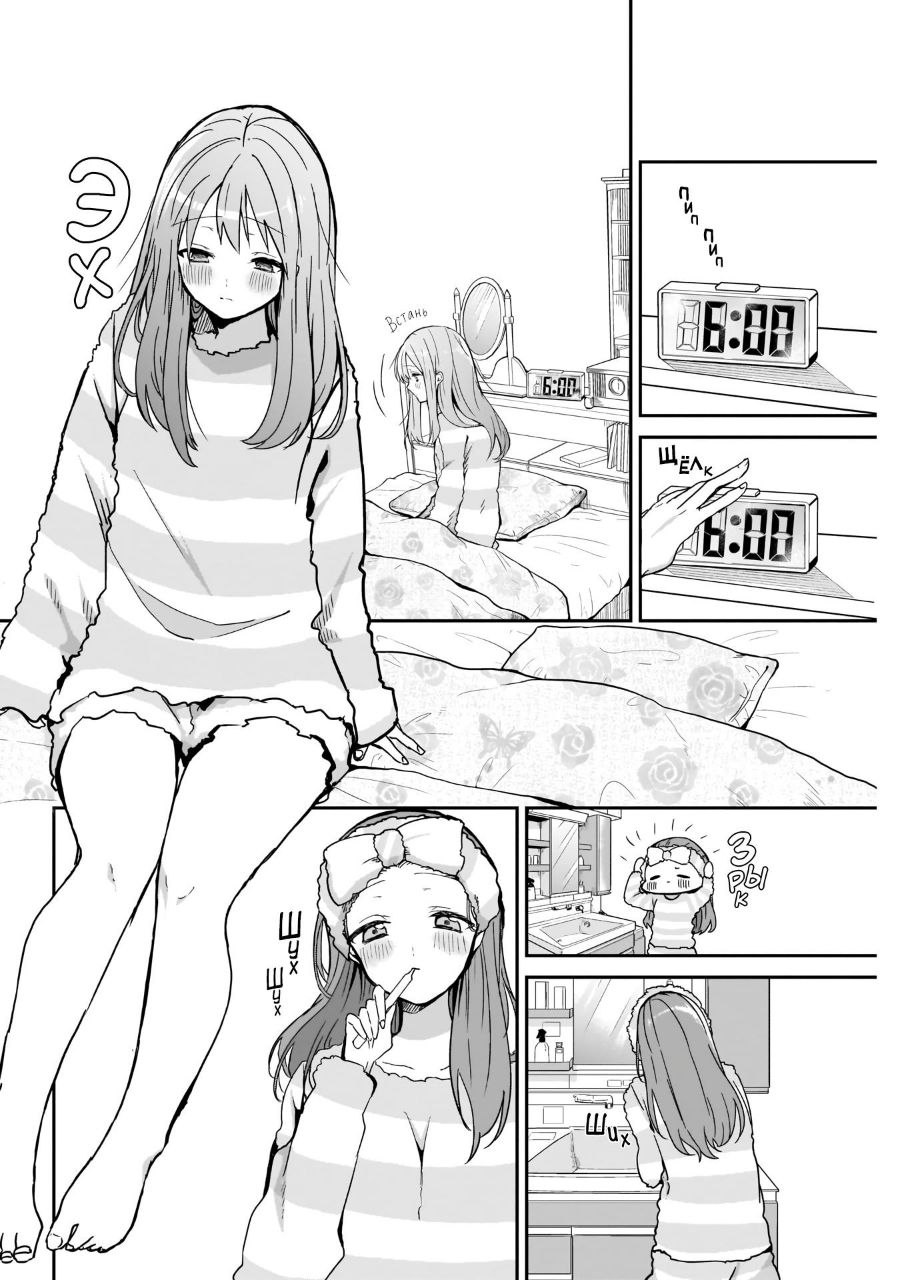
\includegraphics[width=14cm, height=20cm]{аниме2.jpg}
\end{center}
\end{document}  

